\chapter{The Genetic Code}
\label{chap:chapter8}
\minitoc

Up to this point we've used Perl to search for motifs, simulate DNA mutations, generate random sequences, and transcribe DNA to RNA. These are all important activities, and they serve as a good introduction to the computational techniques you can use to study biological systems.

In this chapter, we'll write Perl programs to simulate how the genetic code directs the translation of DNA into protein. I will start by introducing the hash datatype. Then, after a brief discussion of how different data structures (hashes, arrays, and databases) can store and access experimental information, we will write a program to translate DNA to protein. We'll also continue exploring regular expressions and write code to handle FASTA files.

\section{Hashes}
There are three main datatypes in Perl. You've already seen two: scalar variables and arrays. Now we'll start to use the third: \textit{hashes} (also called associative arrays).

A hash provides very fast lookup of the value associated with a key. As an example, say you have a hash called \verb|%english_dictionary|. (Yes, hashes start with the percent sign.) If you want to look up the definition of the word "recreant," you say:

\begin{lstlisting}
$definition = $english_dictionary{'recreant'};
\end{lstlisting}

The scalar \verb|'recreant'| is the key, and the scalar definition that's returned is the value. As you see from this example, hashes (like arrays) change their leading character to a dollar sign when you access a single element, because the value returned from a hash lookup is a scalar value. You can tell a hash lookup from an array element by the type of braces they use: arrays use square brackets [ ]; hashes use curly braces { }.

If you want to assign a value to a key, it's similarly an easy, single statement:

\begin{lstlisting}
$english_dictionary{'recreant'} = "One who calls out in surrender.";
\end{lstlisting}

Also, if you want to initialize a hash with some key-value pairs, it's done much like initializing arrays, but every pair becomes a key-value: 

\begin{lstlisting}
%classification = (
  'dog',      'mammal',
  'robin',    'bird',
  'asp',      'reptile',
);
\end{lstlisting}

which initializes the key \verb|'dog'| with the value \verb|'mammal'|, and so on. There's another way of writing this, which shows what's happening a little more clearly. The following does exactly the same thing as the preceding code, while showing the key-value relationship more clearly: 

\begin{lstlisting}
%classification = (
  'dog'   => 'mammal',
  'robin' => 'bird',
  'asp',  => 'reptile',
);
\end{lstlisting}

You can get an array of all the keys of a hash:

\begin{lstlisting}
@keys  = keys %my_hash;
\end{lstlisting}

You can get an array of all the values of a hash:

\begin{lstlisting}
@values  = values %my_hash;
\end{lstlisting}

You use hashes in lots of different situations, especially when your data is in the form of key-value or you need to look up the value of a key fast. For instance, later in this chapter, we'll develop programs that use hashes to retrieve information about a gene. The gene name is the key; the information about the gene is the value of that key. Mathematically, a Perl hash always represents a finite function.

The name "hash" comes from something called a hash function, which practically any book on algorithms will define, if you've a mind to look it up. Let's skip the details of how they work under the hood and just talk about their behavior. 

\section{Data Structures and Algorithms for Biology}
Biologists explore biological data and try to figure out how to do things with it based on its existing structure in living systems. Bioinformatics is often used to model that existing structure as closely as possible. (Bear with me; I'm speaking in generalities!)

Bioinformatics also can take a slightly different approach. It thinks about what it wants to do with the data and then tries to figure out how to organize it to accomplish that goal. In other words, it tries to produce an algorithm by representing the data in a convenient data structure.

Now that you've got the three datatypes of Perl in hand—namely scalars, arrays, and hashes—it's time to take a look at these interrelated topics of algorithms and data structures. We've already talked about algorithms in \autoref{chap:chapter3}. The present discussion highlights the importance of the organization of the data for algorithms, in other words, the data structures for the algorithm.

The most important point here is that different algorithms often require different data structures. 

\subsection{A Gene Expression Database}
Let's consider a typical problem. Say you're studying an organism that has a total of about 30,000 genes. (Yep, you're right, it's human.) Say you're looking at a type of cell that's never been well characterized under certain interesting environmental conditions, and you are determining, for each gene, whether it's being expressed.\footnote{For the nonbiologists: a gene is expressed when it is transcribed into RNA, so that a protein can be made from it.} You have a nice microarray facility that has given you the expression information for that cell. Now, for each gene, you need to look up whether it's expressed in the cell. You have to put this look-up capability on your web site, so visitors who read your results in your upcoming paper can find the expression data for the genes.

There are several ways to proceed. Let's look at a few alternatives as a short and gentle introduction to the art and science of algorithms and data structures. 

What is your data? For simplicity, let's say you have the names for all the genes in the organism and a number for the expressed genes indicating the level of the expression in your experiment; the unexpressed genes have the number 0.

\subsection{Gene Expression Data Using Unsorted Arrays}
Now let's suppose you want to know if the genes were expressed, but not the expression levels, and you want to solve this programming problem using arrays. After all, you are somewhat familiar with arrays by this point. How do you proceed?

You might store in the array only the names of the genes that are being expressed and discard the other gene names. Say there were 8,000 expressed genes. Then, for any query, the answer requires looking through the array and comparing the query with each gene in the array until either you find it or get to the end of the array without finding it.

That works, but there are problems. Mainly, it's kind of slow. This isn't bad if you just do it now and then, but if you've got a lot of people hitting your web site asking questions about this new expression data, it can be a problem. On average, a lookup for an expressed gene requires looking through 4,000 gene names. A lookup for an unexpressed gene takes 8,000 comparisons.

Also, if someone asked about a gene missing from your study, you couldn't respond, since you discarded the unexpressed gene names. The query gives a negative response, not an error message saying the gene being searched for isn't part of your experiment. This might even be a false negative if the query gene that wasn't part of your study actually is expressed in the cell type (but you just missed it). You'd prefer it if your program would report to the user that no gene by that name was studied.

So you decide to keep all 30,000 genes in the array. (Of course, now a search will be slower.) But how to distinguish the expressed from the unexpressed genes? You can load each gene's name into the array and then append the expression measurement after the name of each gene. Then you will definitely know if a gene is missing from your experiment.

However, the program is still a bit slow. You still have to search through the entire array until you find the gene or determine that it wasn't studied. You may find it right away if it's the first element in the array, or you may have to wait until the last element. On average, you have to search through half of the array. Plus, you have to compare the name of the searched-for gene with the names of the genes in the array one by one. It will average 15,000 comparisons per query: slow.  (Actually, on a modern computer, not too horribly slow, really, but I'm making a point. These sorts of things do add up with a program that runs too slowly.)

Another problem is that you're now keeping two values in one scalar: the gene name and the expression measurement. To do anything with this data, you have to also separate the gene name from the measurement of the expression of the gene.

Despite these drawbacks, this method will work. Now, let's think about alternatives. 

\subsection{Gene Expression Data Using Sorted Arrays and Binary Search}
You might try storing all the gene names in alphabetical order in the array and then use the following search technique. First, look at the middle element. (You can tell the size of the array, as we've seen, with the expression \verb|scalar @array|). If your gene name is before that middle element alphabetically, you ignore the second half of the array and pick the middle element of the remaining half of the array. You continue, at each step narrowing the search to half the previous number of elements, until you find a match or discover there is none. Here it is in pseudocode: 

\begin{lstlisting}
Given a sorted array, and an element:

Until you find the element or discover it's not there,

  Pick the midpoint of the array, $array[scalar(@array)/2]

  Compare your element with the element at the midpoint

  If that matches your element, you're done.

  Else, ignore the half of the array that your element is not in
}
\end{lstlisting}

To compare two strings alphabetically in Perl, you use the \textit{cmp} operator, which returns 0 if the two strings are the same, -1 if they are in alphabetical order, and 1 if they are in reverse alphabetical order. For example, the following returns 0:

\begin{lstlisting}
'ZZZ' cmp 'ZZZ';
\end{lstlisting}

This returns -1:

\begin{lstlisting}
'AAA' cmp 'ZZZ';
\end{lstlisting}

Finally, this returns 1:

\begin{lstlisting}
'ZZZ' cmp 'AAA';
\end{lstlisting}

This algorithm is called a \textit{binary search}, and it considerably speeds up the process of searching in an array, for example, to search 30,000 genes takes only about 15 times through the loop, maximum. (As compared to 15,000 comparisons, average, for the unsorted array.) Of course, you also have to sort the list, which might take awhile. If you need to keep adding elements, you have to either insert them in the right place or add them to the end and sort the array again. All that inserting or sorting might slow things down considerably. But if you're just sorting it once and then doing lots of lookups, a binary search might be worth doing.

While we're at it, let's look at how to sort an array. Here's how to sort an array of strings alphabetically:

\begin{lstlisting}
@array = sort @array;
\end{lstlisting}

Here's how to sort an array of numbers in ascending order:

\begin{lstlisting}
@array = sort { $a <=> $b  } @array;
\end{lstlisting}

Many other kinds of sorting can be done, but these are the most common. For more details, see the Perl documentation for the \textit{sort} function. 

\subsection{Gene Expression Data Using Hashes}
You can also use hashes to find a gene in your data. To do so, you can load the hash so that the keys are the gene names and the values are the expression measurement. Then a single call on the hash, with the name of the desired gene as a key, returns the results of the experiment for that gene, and you've got your answer. This process is also cleaner than storing the gene name and the expression result in one scalar string; here the key is a scalar, and the value is a separate scalar.

Furthermore, due to how hashes are made, you get an answer back very quickly, because decent hashes don't have to search hard to find the value of a key. Using hashes is typically faster than binary searches. Plus, you'd know if the gene being searched for was in the data, because you can explicitly ask if a hash value is defined by saying something like:

\begin{lstlisting}
if( defined $myhash{'mykey'}  ) { ... }
\end{lstlisting}

Also, you'll get an error message if you have warnings turned on, and you refer to an undefined value.

Another advantage of hashes over binary searching is that you can add or subtract elements to hashes without resorting the entire array.

Finally, because hashes are built into Perl as a basic datatype, they are easy to use, and you won't have to do much programming to accomplish your goal. It is usually the case that it's more important to save time writing a program then it is to save time running it. I mention this in \autoref{chap:chapter3}, but it's worth emphasizing. To a programmer, the lazy way is often the most efficient way: let the machine do the work!

Don't get the idea that hashes are always the right way to go, however. For instance, they don't store their elements in a sorted order, so if you need to look at the data that way, you have to explicitly sort it, like so:

\begin{lstlisting}
@sorted_keys = sort keys %my_hash;
\end{lstlisting}

This is do-able, but it can be a bit slow on a large array. (You could also sort the values, of course.)

To conclude the discussion of data structures for our expression data example, here's an informal survey of the properties of some different data structures in Perl for searching, adding and deleting, and maintaining sorted order in a set of gene names: 

\begin{itemize}
  \item Use a hash if you just need to see if something is in a set and don't need to list the set in order.
  \item A sorted array combined with a binary search algorithm will do if you need an ordered set and pretty fast lookup and don't need to add or subtract elements very often.
  \item An array, in conjunction with the Perl functions \textit{push} and \textit{pop}, works well if you don't need to sort the elements but do need to quickly get at the most recently added element.
  \item A Perl array with the functions \textit{push} and \textit{shift} will serve if you don't need the elements sorted but need to add elements. It's especially useful to always remove the "oldest" element (the element that has been in the array the longest).
\end{itemize}

For more information, see \autoref{chap:chapteraa} and especially \textit{Mastering Algorithms with Perl} (published by O'Reilly). 

\subsection{Relational Databases}
Databases are programs that store and retrieve large amounts of data. They provide the most common forms of datatypes to use in algorithms. There are several popular databases. Some good ones that are free of charge (the best ones are very expensive), and Perl provides access to all the most popular ones. The Perl/DBI modules, for instance, provide convenient access to relational databases from Perl programs.

Most databases are called relational, which describes how they store data. Another common name for these types of databases is \textit{relational database management systems}, or RDMS. 

Relational databases store data organized in tables. The data is usually entered and extracted with a query language called \textit{Structured Query Language}, or SQL, which is a fairly simple language for accessing the data in the tables and following links between the tables.

Relational databases are the most popular way to store and retrieve large amounts of data, but they do require a fair bit of learning. Programming with relational databases is beyond the scope of this book, but if you end up doing a lot of programming with Perl, you'll find that knowing the basics of using a database is a valuable skill. See the discussion in \autoref{chap:chapter13}.

In particular, it's perfectly reasonable to store your gene expression data in a relational database and use that in your program to respond to queries made on your web site. 

\subsection{DBM}
Perl has a simple, built-in way to store hash data, called \textit{database management} (DBM). It's simple to use: after starting up, it "ties" a hash to a file on your computer disk, so you can save a hash to reuse at a later date. This is, in effect, a simple (and very useful) database. Apart from the initialization, you use it as you would any other hash. You can store your genes and expression data in a DBM file and then use it as a hash. There's more on DBM in \autoref{chap:chapter10}.

\section{The Genetic Code}
The genetic code is how a cell translates the information contained in its DNA into amino acids and then proteins, which do the real work in the cell.

\subsection{Background}
Herein is a short introduction for the nonbiologists.

As stated earlier, DNA encodes the primary structure (i.e., the amino acid sequence) of proteins. DNA has four nucleotides, and proteins have 20 amino acids. The encoding works by taking each group of three nucleotides from the DNA and "translating" them to an amino acid or a stop signal. Each group of three nucleotides is called a \textit{codon}. We'll see in detail how this coding and translation works.

Actually, \textit{transcription} first uses DNA to make RNA, and then \textit{translation} uses RNA to make proteins. This is called the \textit{central dogma} of molecular biology. But in this course, I'll abbreviate the process and somewhat inaccurately call the entire process from DNA to protein "translation."

The reason for this cavalier distinction is that the whole business is much easier to simulate on computer using strings to represent the DNA, RNA, and proteins. In fact, as shown in \autoref{chap:chapter4}, transcribing DNA to RNA is very easy indeed. In your computer simulations, you can simply skip that step, since it's just a matter of changing one letter to another. (The actual process in the cell, of course, is much more complex.)

Note that with four kinds of bases, each group of three bases of DNA can represent as many as 4 x 4 x 4 = 64 possible amino acids. Since there are only 20 amino acids plus a stop signal, the genetic code has evolved some redundancy, so that some amino acids are represented by more than one codon. Every possible three bases of DNA—each codon—represents some amino acid (apart from the three codons that represent a stop signal). 

The chart in \autoref{fig:figure8.1} shows how the various bases combine to form amino acids. There are many interesting things to note about the genetic code. For our purposes, the most important is redundancy—the way more than one codon translates to the same amino acid. We'll program this using character classes and regular expressions, as you'll soon see.\footnote{Also note that the genetic code in \autoref{fig:figure8.1} is properly based on RNA, where uracil appears instead of thymine. In our programs, we're going to go directly from DNA to amino acids, so our codons will use thymine instead of uracil.}

\begin{figure}
  \centering
  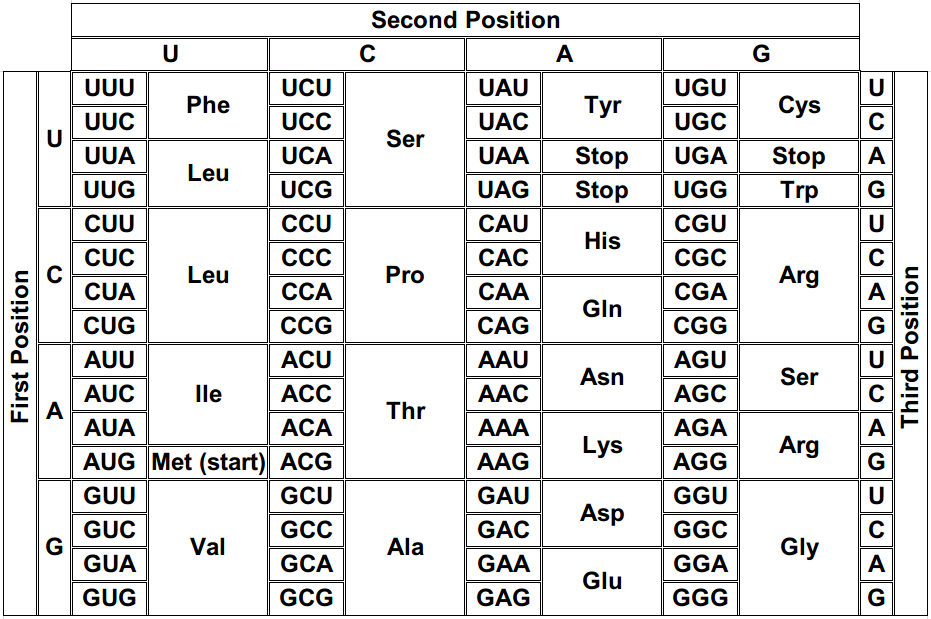
\includegraphics[width=13cm]{figure8.1.png}
  \caption{The genetic code}
  \label{fig:figure8.1}
\end{figure}

The machinery of the cell actually starts at some point along the RNA and "reads" the sequences codon after codon, attaching the encoded amino acid to the end of the growing protein sequence.  \autoref{exam:example8.1} simulates this, reading the string of DNA three bases at a time and concatenating the symbol for the encoded amino acid to the end of the growing protein string. In the cell, the process stops when one of the three stop codons is encountered. 

\subsection{Translating Codons to Amino Acids}
The first task is to enable the following programs to do the translation from the three-nucleotide codons to the amino acids. This is the most important step in implementing the genetic code, which is the encoding of amino acids by three-nucleotide codons.

Here's a subroutine that returns an amino acid (represented by a one-letter abbreviation) given a three-letter DNA codon: 

\begin{lstlisting}
# codon2aa
#
# A subroutine to translate a DNA 3-character codon to an amino acid

sub codon2aa {
  my($codon) = @_;
   
     if ( $codon =~ /TCA/i )   { return 'S' }   # Serine
  elsif ( $codon =~ /TCC/i )   { return 'S' }   # Serine
  elsif ( $codon =~ /TCG/i )   { return 'S' }   # Serine
  elsif ( $codon =~ /TCT/i )   { return 'S' }   # Serine
  elsif ( $codon =~ /TTC/i )   { return 'F' }   # Phenylalanine
  elsif ( $codon =~ /TTT/i )   { return 'F' }   # Phenylalanine
  elsif ( $codon =~ /TTA/i )   { return 'L' }   # Leucine
  elsif ( $codon =~ /TTG/i )   { return 'L' }   # Leucine
  elsif ( $codon =~ /TAC/i )   { return 'Y' }   # Tyrosine
  elsif ( $codon =~ /TAT/i )   { return 'Y' }   # Tyrosine
  elsif ( $codon =~ /TAA/i )   { return '_' }   # Stop
  elsif ( $codon =~ /TAG/i )   { return '_' }   # Stop
  elsif ( $codon =~ /TGC/i )   { return 'C' }   # Cysteine
  elsif ( $codon =~ /TGT/i )   { return 'C' }   # Cysteine
  elsif ( $codon =~ /TGA/i )   { return '_' }   # Stop
  elsif ( $codon =~ /TGG/i )   { return 'W' }   # Tryptophan
  elsif ( $codon =~ /CTA/i )   { return 'L' }   # Leucine
  elsif ( $codon =~ /CTC/i )   { return 'L' }   # Leucine
  elsif ( $codon =~ /CTG/i )   { return 'L' }   # Leucine
  elsif ( $codon =~ /CTT/i )   { return 'L' }   # Leucine
  elsif ( $codon =~ /CCA/i )   { return 'P' }   # Proline
  elsif ( $codon =~ /CCC/i )   { return 'P' }   # Proline
  elsif ( $codon =~ /CCG/i )   { return 'P' }   # Proline
  elsif ( $codon =~ /CCT/i )   { return 'P' }   # Proline
  elsif ( $codon =~ /CAC/i )   { return 'H' }   # Histidine
  elsif ( $codon =~ /CAT/i )   { return 'H' }   # Histidine
  elsif ( $codon =~ /CAA/i )   { return 'Q' }   # Glutamine
  elsif ( $codon =~ /CAG/i )   { return 'Q' }   # Glutamine
  elsif ( $codon =~ /CGA/i )   { return 'R' }   # Arginine
  elsif ( $codon =~ /CGC/i )   { return 'R' }   # Arginine
  elsif ( $codon =~ /CGG/i )   { return 'R' }   # Arginine
  elsif ( $codon =~ /CGT/i )   { return 'R' }   # Arginine
  elsif ( $codon =~ /ATA/i )   { return 'I' }   # Isoleucine
  elsif ( $codon =~ /ATC/i )   { return 'I' }   # Isoleucine
  elsif ( $codon =~ /ATT/i )   { return 'I' }   # Isoleucine
  elsif ( $codon =~ /ATG/i )   { return 'M' }   # Methionine
  elsif ( $codon =~ /ACA/i )   { return 'T' }   # Threonine
  elsif ( $codon =~ /ACC/i )   { return 'T' }   # Threonine
  elsif ( $codon =~ /ACG/i )   { return 'T' }   # Threonine
  elsif ( $codon =~ /ACT/i )   { return 'T' }   # Threonine
  elsif ( $codon =~ /AAC/i )   { return 'N' }   # Asparagine
  elsif ( $codon =~ /AAT/i )   { return 'N' }   # Asparagine
  elsif ( $codon =~ /AAA/i )   { return 'K' }   # Lysine
  elsif ( $codon =~ /AAG/i )   { return 'K' }   # Lysine
  elsif ( $codon =~ /AGC/i )   { return 'S' }   # Serine
  elsif ( $codon =~ /AGT/i )   { return 'S' }   # Serine
  elsif ( $codon =~ /AGA/i )   { return 'R' }   # Arginine
  elsif ( $codon =~ /AGG/i )   { return 'R' }   # Arginine
  elsif ( $codon =~ /GTA/i )   { return 'V' }   # Valine
  elsif ( $codon =~ /GTC/i )   { return 'V' }   # Valine
  elsif ( $codon =~ /GTG/i )   { return 'V' }   # Valine
  elsif ( $codon =~ /GTT/i )   { return 'V' }   # Valine
  elsif ( $codon =~ /GCA/i )   { return 'A' }   # Alanine
  elsif ( $codon =~ /GCC/i )   { return 'A' }   # Alanine
  elsif ( $codon =~ /GCG/i )   { return 'A' }   # Alanine
  elsif ( $codon =~ /GCT/i )   { return 'A' }   # Alanine
  elsif ( $codon =~ /GAC/i )   { return 'D' }   # Aspartic Acid
  elsif ( $codon =~ /GAT/i )   { return 'D' }   # Aspartic Acid
  elsif ( $codon =~ /GAA/i )   { return 'E' }   # Glutamic Acid
  elsif ( $codon =~ /GAG/i )   { return 'E' }   # Glutamic Acid
  elsif ( $codon =~ /GGA/i )   { return 'G' }   # Glycine
  elsif ( $codon =~ /GGC/i )   { return 'G' }   # Glycine
  elsif ( $codon =~ /GGG/i )   { return 'G' }   # Glycine
  elsif ( $codon =~ /GGT/i )   { return 'G' }   # Glycine
  else {
   print STDERR "Bad codon \"$codon\"!!\n";
   exit;
  }
}
\end{lstlisting}

This code is clear and simple, and the layout makes it obvious what's happening. However, it can take a while to run. For instance, given the codon GGT for glycine, it has to check each test until it finally succeeds on the last one, and that's a lot of string comparisons. Still, the code achieves its purpose.

There's something new happening in the code's error message. Recall filehandles from \autoref{chap:chapter4} and how they access data in files. From \autoref{chap:chapter5}, remember the special filehandle STDIN that reads user input from the keyboard. STDOUT and STDERR are also special filehandles that are always available to Perl programs. STDOUT directs output to the screen (usually) or another standard place. When a filehandle is missing from a \verb|print| statement, STDOUT is assumed. The \textit{print} statement accepts a filehandle as an optional argument, but so far, we've been printing to the default STDOUT. Here, error messages are directed to STDERR, which usually prints to the screen, but on many computer systems they can be directed to a special error file or other location. Alternatively, you sometimes want to direct STDOUT to a file or elsewhere but want STDERR error messages to appear on your screen. I mention these options because you are likely to come across them in Perl code; we don't use them much in this book (see \autoref{chap:chapterab} for more information).  

\subsection{The Redundancy of the Genetic Code}
I've remarked on the redundancy of the genetic code, and the last subroutine clearly displays this redundancy. It might be interesting to express that in your subroutine. Notice that groups of redundant codons almost always have the same first and second bases and vary in the third. You've used character classes in regular expressions to match any of a set of characters. Now, let's try to redo the subroutine to make one test for each redundant group of codons: 

\begin{lstlisting}
# codon2aa
#
# A subroutine to translate a DNA 3-character codon to an amino acid
#   Version 2

sub codon2aa {
  my($codon) = @_;
 
     if ( $codon =~ /GC./i)        { return 'A' }    # Alanine
  elsif ( $codon =~ /TG[TC]/i)     { return 'C' }    # Cysteine
  elsif ( $codon =~ /GA[TC]/i)     { return 'D' }    # Aspartic Acid
  elsif ( $codon =~ /GA[AG]/i)     { return 'E' }    # Glutamic Acid
  elsif ( $codon =~ /TT[TC]/i)     { return 'F' }    # Phenylalanine
  elsif ( $codon =~ /GG./i)        { return 'G' }    # Glycine
  elsif ( $codon =~ /CA[TC]/i)     { return 'H' }    # Histidine
  elsif ( $codon =~ /AT[TCA]/i)    { return 'I' }    # Isoleucine
  elsif ( $codon =~ /AA[AG]/i)     { return 'K' }    # Lysine
  elsif ( $codon =~ /TT[AG]|CT./i) { return 'L' }    # Leucine
  elsif ( $codon =~ /ATG/i)        { return 'M' }    # Methionine
  elsif ( $codon =~ /AA[TC]/i)     { return 'N' }    # Asparagine
  elsif ( $codon =~ /CC./i)        { return 'P' }    # Proline
  elsif ( $codon =~ /CA[AG]/i)     { return 'Q' }    # Glutamine
  elsif ( $codon =~ /CG.|AG[AG]/i) { return 'R' }    # Arginine
  elsif ( $codon =~ /TC.|AG[TC]/i) { return 'S' }    # Serine
  elsif ( $codon =~ /AC./i)        { return 'T' }    # Threonine
  elsif ( $codon =~ /GT./i)        { return 'V' }    # Valine
  elsif ( $codon =~ /TGG/i)        { return 'W' }    # Tryptophan
  elsif ( $codon =~ /TA[TC]/i)     { return 'Y' }    # Tyrosine
  elsif ( $codon =~ /TA[AG]|TGA/i) { return '_' }    # Stop
  else {
    print STDERR "Bad codon \"$codon\"!!\n";
    exit;
  }
}
\end{lstlisting}

Using character classes and regular expressions, this code clearly shows the redundancy of the genetic code. Also notice that the one-character codes for the amino acids are now in alphabetical order. 

A character class such as \verb|[TC]| matches a single character, either T or C. The \verb|.| is the regular expression that matches any character except a newline. The \verb|/GT./i| expression for valine matches GTA, GTC, GTG, and GTT, all of which are codons for valine. (Of course, the period matches any other character, but the \verb|$codon| is assumed to have only A,C,G, or T characters.) The i after the regular expression means match uppercase or lowercase, for instance \verb|/T/i| matches T or t.

The new feature in these regular expressions is the use of the vertical bar or pipe (|) to separate two choices. Thus for serine, \verb=/TC.|AG[TC]/= matches \verb|/TC./| or \verb|/AG[TC]/|. In this program, you need only two choices per regular expression, but you can use as many vertical bars as you like.

You can also group parts of a regular expression in parentheses, and use vertical bars in them. For example, \verb=/give me a (break|meal)/= matches "give me a break" or "give me a meal." 

\subsection{Using Hashes for the Genetic Code}
If you think about using a hash for this translation, you'll see it's a natural way to proceed. For each codon key the amino acid value is returned. Here's the code: 

\begin{lstlisting}
#
# codon2aa
#
# A subroutine to translate a DNA 3-character codon to an amino acid
#   Version 3, using hash lookup

sub codon2aa {
  my($codon) = @_;

  $codon = uc $codon;
 
  my(%genetic_code) = (
  
  'TCA' => 'S',    # Serine
  'TCC' => 'S',    # Serine
  'TCG' => 'S',    # Serine
  'TCT' => 'S',    # Serine
  'TTC' => 'F',    # Phenylalanine
  'TTT' => 'F',    # Phenylalanine
  'TTA' => 'L',    # Leucine
  'TTG' => 'L',    # Leucine
  'TAC' => 'Y',    # Tyrosine
  'TAT' => 'Y',    # Tyrosine
  'TAA' => '_',    # Stop
  'TAG' => '_',    # Stop
  'TGC' => 'C',    # Cysteine
  'TGT' => 'C',    # Cysteine
  'TGA' => '_',    # Stop
  'TGG' => 'W',    # Tryptophan
  'CTA' => 'L',    # Leucine
  'CTC' => 'L',    # Leucine
  'CTG' => 'L',    # Leucine
  'CTT' => 'L',    # Leucine
  'CCA' => 'P',    # Proline
  'CCC' => 'P',    # Proline
  'CCG' => 'P',    # Proline
  'CCT' => 'P',    # Proline
  'CAC' => 'H',    # Histidine
  'CAT' => 'H',    # Histidine
  'CAA' => 'Q',    # Glutamine
  'CAG' => 'Q',    # Glutamine
  'CGA' => 'R',    # Arginine
  'CGC' => 'R',    # Arginine
  'CGG' => 'R',    # Arginine
  'CGT' => 'R',    # Arginine
  'ATA' => 'I',    # Isoleucine
  'ATC' => 'I',    # Isoleucine
  'ATT' => 'I',    # Isoleucine
  'ATG' => 'M',    # Methionine
  'ACA' => 'T',    # Threonine
  'ACC' => 'T',    # Threonine
  'ACG' => 'T',    # Threonine
  'ACT' => 'T',    # Threonine
  'AAC' => 'N',    # Asparagine
  'AAT' => 'N',    # Asparagine
  'AAA' => 'K',    # Lysine
  'AAG' => 'K',    # Lysine
  'AGC' => 'S',    # Serine
  'AGT' => 'S',    # Serine
  'AGA' => 'R',    # Arginine
  'AGG' => 'R',    # Arginine
  'GTA' => 'V',    # Valine
  'GTC' => 'V',    # Valine
  'GTG' => 'V',    # Valine
  'GTT' => 'V',    # Valine
  'GCA' => 'A',    # Alanine
  'GCC' => 'A',    # Alanine
  'GCG' => 'A',    # Alanine
  'GCT' => 'A',    # Alanine
  'GAC' => 'D',    # Aspartic Acid
  'GAT' => 'D',    # Aspartic Acid
  'GAA' => 'E',    # Glutamic Acid
  'GAG' => 'E',    # Glutamic Acid
  'GGA' => 'G',    # Glycine
  'GGC' => 'G',    # Glycine
  'GGG' => 'G',    # Glycine
  'GGT' => 'G',    # Glycine
  );

  if(exists $genetic_code{$codon}) {
    return $genetic_code{$codon};
  }else{

    print STDERR "Bad codon \"$codon\"!!\n";
    exit;
  }
}
\end{lstlisting}

This subroutine is simple: it initializes a hash and then performs a single lookup of its single argument in the hash. The hash has 64 keys, one for each codon.

Notice there's a function \textit{exists} that returns \verb|true| if the key \verb|$codon| exists in the hash. It's equivalent to the \textit{else} statement in the two previous versions of the \textit{codon2aa} subroutine.\footnote{A key might exist in a hash, but its value can be undefined. The \textit{defined} function checks for defined values. Also, of course, the value might be 0 or the empty string, in which case, it fails a test such as \verb|if ($hash{$key})| because, even though the key exists and the value is defined, the value evaluates to \verb|false| in a conditional test.}

Also notice that to make this subroutine work on lowercase DNA as well as uppercase, you translate the incoming argument into uppercase to match the data in the \verb|%genetic_code| hash. You can't give a regular expression to a hash as a key; it must be a simple scalar value, such as a string or a number, so the case translation must be done first. (Alternatively, you can make the hash twice as big.) Similarly, character classes don't work in the keys for hashes, so you have to specify each one of the 64 codons individually.

You may wonder why bother wrapping this last bit of code in a subroutine at all. Why not just declare and initialize the hash and do the lookups directly in the hash instead of going through the subroutine? Well, the subroutine does do a little bit of error checking for nonexistent keys, so having a subroutine saves doing that error checking yourself each time you use the hash.

Additionally, wrapping the code in a subroutine gives a little insurance for the future. If all the code you write does codon translation by means of our subroutine, it would be simplicity itself to switch over to a new way of doing the translation. Perhaps a new kind of datatype will be added to Perl in the future, or perhaps you want to do lookups from a database or a DBM file. Then all you have to do is change the internals of this one subroutine. As long as the interface to the subroutine remains the same—that is to say, as long as it still takes one codon as an argument and returns a one-character amino acid—you don't need to worry about how it accomplishes the translation from the standpoint of the rest of the programs. Our subroutine has become a \textit{black box}. This is one significant benefit of modularization and organization of programs with subroutines. 

There's another good, and biological, reason why you should use a subroutine for the genetic code. There is actually more than one genetic code, because there are differences as to how DNA encodes amino acids among mammals, plants, insects, and yeast—especially in the mitochondria. So if you have modularized the genetic code, you can easily modify your program to work with a range of organisms.

One of the benefits of hashes is that they are fast. Unfortunately, our subroutine declares the whole hash each time the subroutine is called, even for one lookup. This isn't so efficient; in fact, it's kind of slow. There are other, much faster ways that involve declaring the genetic code hash only once as a global variable, but they would take us a little far afield at this point. Our current version has the advantage of being easy to read. So, let's be officially happy with the hash version of \textit{codon2aa} and put it into our module in the file \textit{BeginPerlBioinfo.pm} (see \autoref{chap:chapter6}).

Now that we've got a satisfactory way to translate codons to amino acids, we'll start to use it in the next section and in the examples. 

\section{Translating DNA into Proteins}
\autoref{exam:example8.1} shows how the new \textit{codon2aa} subroutine translates a whole DNA sequence into protein. 

%\textbf{Example 8-1. Translate DNA into protein }
\lstinputlisting[label=exam:example8.1,caption={Example 8.1. Translate DNA into protein }]{./scripts/example8-1.pl}

To make this work, you'll need the \textit{BeginPerlBioinfo.pm} module for your subroutines in a separate file the program can find, as discussed in \autoref{chap:chapter6}. You also have to add the \textit{codon2aa} subroutine to it. Alternatively, you can add the code for the subroutine \textit{condon2aa} directly to the program in \autoref{exam:example8.1} and remove the reference to the \textit{BeginPerlBioinfo.pm} module.

Here's the output from \autoref{exam:example8.1}:

\begin{lstlisting}
I translated the DNA

CGACGTCTTCGTACGGGACTAGCTCGTGTCGGTCGC

  into the protein

RRLRTGLARVGR
\end{lstlisting}

You've seen all the elements in \autoref{exam:example8.1} before, except for the way it loops through the DNA with this statement:

\begin{lstlisting}
for(my $i=0; $i < (length($dna) - 2) ; $i += 3) {
\end{lstlisting}

Recall that a \verb|for| loop has three parts, delimited by the two semicolons. The first part initializes a counter: \verb|my $i=0| statically scopes the \verb|$i| variable so it's visible only inside this block, and any other \verb|$i| elsewhere in the code (well, in this case, there aren't any, but it can happen) is now invisible inside the block. The third part of the \verb|for| loop increments the counter after all the statements in the block are executed and before returning to the beginning of the loop:

\begin{lstlisting}
$i += 3
\end{lstlisting}

Since you're trying to march through the DNA three bases at a shot, you increment by three.

The second, middle part of the \verb|for| loop tests whether the loop should continue:

\begin{lstlisting}
$i < (length($dna) - 2)
\end{lstlisting}

The point is that if there are none, one, or two bases left, you should quit, because there's not enough to make a codon. Now, the positions in a string of DNA of a certain length are numbered from \verb|0| to \verb|length-1|. So if the position counter \verb|$i| has reached \verb|length-2|, there's only two more bases (at positions \verb|length-2| and \verb|length-1|), and you should quit. Only if the position counter \verb|$i| is less than \verb|length-2| will you still have at least three bases left, enough for a codon. So the test succeeds only if:

\begin{lstlisting}
$i < (length($dna) -2)
\end{lstlisting}

(Notice also how the whole expression to the right of the less-than sign is enclosed in parentheses; we'll discuss this in \autoref{chap:chapter9} in \autoref{sect:section9.3.1})

The line of code:

\begin{lstlisting}
$codon = substr ($dna, $i 3);
\end{lstlisting}

actually extracts the 3-base codon from the DNA. The call to the \verb|substr| function specifies a substring of \verb|$dna| at position \verb|$i| of length \verb|3|, and saves it in the variable \verb|$codon|. 

If you know you'll need to do this DNA-to-protein translation a lot, you can turn \autoref{exam:example8.1} into a subroutine. Whenever you write a subroutine, you have to think about which arguments you may want to give the subroutine. So you realize, there may come a time when you'll have some large DNA sequence but only want to translate a given part of it. Should you add two arguments to the subroutine as beginning and end points? You could, but decide not to. It's a judgment call—part of the art of decomposing a collection of code into useful fragments. But it might be better to have a subroutine that just translates; then you can make it part of a larger subroutine that picks endpoints in the sequence, if needed. The thinking is that you'll usually just translate the whole thing and always typing in \verb|0| for the start and \verb|length($dna)-1| at the end, would be an annoyance. Of course, this depends on what you're doing, so this particular choice just illustrates your thinking when you write the code.

You should also remove the informative \verb|print| statement at the end, because it's more suited to a main program than a subroutine.

Anyway, you've now thought through the design and just want a subroutine that takes one argument containing DNA and returns a peptide translation: 

\begin{lstlisting}
# dna2peptide 
#
# A subroutine to translate DNA sequence into a peptide

sub dna2peptide {
  
  my($dna) = @_;

  use strict;
  use warnings;
  use BeginPerlBioinfo;     # see Chapter 6 about this module

  # Initialize variables
  my $protein = '';

  # Translate each three-base codon to an amino acid, and append to a protein 
  for(my $i=0; $i < (length($dna) - 2) ; $i += 3) {
    $protein .= codon2aa( substr($dna,$i,3));
  }

  return $protein;
  }
\end{lstlisting}

Now add subroutine \textit{dna2peptide} to the \textit{BeginPerlBioinfo.pm} module.

Notice that you've eliminated one of the variables in making the subroutine out of \autoref{exam:example8.1}: the variable \verb|$codon|. Why?

Well, one reason is because you can. In \autoref{exam:example8.1}, you were using \textit{substr} to extract the codon from \verb|$dna|, saving it in variable \verb|$codon| and then passing it into the subroutine \textit{codon2aa}. This new way eliminates the middleman. Put the call to \textit{substr} that extracts the codon as the argument to the subroutine \textit{codon2aa} so that the value is passed in just as before, but without having to copy it to the variable \verb|$codon| first. 

This has somewhat improved efficiency and speed. Since copying strings is one of the slower things computer programs do, eliminating a bunch of string copies is an easy and effective way to speed up a program.

But has it made the program less readable? You be the judge. I think it has, a little, but the comment right before the loop seems to make everything clear enough, for me, anyway. It's important to have readable code, so if you really need to boost the speed of a subroutine, but find it makes the code harder to read, be sure to include enough comments for the reader to be able to understand what's going on.

For the first time \textit{use} function calls are being included in a subroutine instead of the main program:

\begin{lstlisting}
use strict;
use warnings;
use BeginPerlBioinfo;
\end{lstlisting}

This may be redundant with the calls in the main program, but it doesn't do any harm (Perl checks and loads a module only once). If this subroutine should be called from a module that doesn't already load the modules, it's done some good after all.

Now let's improve how we deal with DNA in files. 

\section{Reading DNA from Files in FASTA Format}
Over the fairly short history of bioinformatics, several different biologists and programmers invented several ways to format sequence data in computer files, and so bioinformaticians must deal with these different formats. We need to extract the sequence data and the annotations from these files, which requires writing code to deal with each different format.

There are many such formats, perhaps as many as 20 in regular use for DNA alone. The very multiplicity of these formats can be an annoyance when you're analyzing a sequence in the lab: it becomes necessary to translate from one format to another for the various programs you use to examine the sequence. Here are some of the most popular: 

\textcolor{red}{\textit{FASTA}}
\begin{adjustwidth}{2em}{}
The FASTA and Basic Local Alignment Search Technique (BLAST) programs are popular; they both use the FASTA format. Because of its simplicity, the FASTA format is perhaps the most widely used of all formats, aside from GenBank. 
\end{adjustwidth}

\textcolor{red}{\textit{Genetic Sequence Data Bank (GenBank)}}
\begin{adjustwidth}{2em}{}
GenBank is a collection of all publicly released genetic data. It includes lots of information in addition to the DNA sequence. It's very important, and we'll be looking closely at GenBank files in \autoref{chap:chapter10}. 
\end{adjustwidth}

\textcolor{red}{\textit{European Molecular Biology Laboratory (EMBL)}}
\begin{adjustwidth}{2em}{}
The EMBL database has substantially the same data as the GenBank and the DDBJ (DNA Data Bank of Japan), but the format is somewhat different. 
\end{adjustwidth}

\textcolor{red}{\textit{Simple data, or Applied Biosystems (ABI) sequencer output}}
\begin{adjustwidth}{2em}{}
This is DNA sequence data that has no formatting whatsoever, just the characters that represent the bases; it is output into files by the sequencing machines from ABI and from other machines and programs. 
\end{adjustwidth}

\textcolor{red}{\textit{Protein Identification Resource (PIR)}}
\begin{adjustwidth}{2em}{}
PIR is a well-curated collection of protein sequence data.
\end{adjustwidth}

\textcolor{red}{\textit{Genetics Computer Group (GCG)}}
\begin{adjustwidth}{2em}{}
The GCG program (a.k.a. the GCG Wisconsin package) from Accelrys is used at many large research institutions. Data must be in GCG format to be usable by their programs. 
\end{adjustwidth}

Of these six sequence formats, GenBank and FASTA are by far the most common. The next few sections take you through the process of reading and manipulating data in FASTA. 

\subsection{FASTA Format}
Let's write a subroutine that can handle FASTA-style data. This is useful in its own right and as a warm-up for the upcoming chapters on GenBank, PDB, and BLAST.

FASTA format is basically just lines of sequence data with newlines at the end so it can be printed on a page or displayed on a computer screen. The length of the lines isn't specified, but for compatibility, it's best to limit them to 80 characters in length. There is also \textit{header information}, a line or lines at the beginning of the file that start with the greater-than > character, that can contain any text whatsoever (or no text). Typically, a header line contains the name of the DNA or the gene it comes from, often separated by a vertical bar from additional information about the sequence, the experiment that produced it, or other, nonsequence information of that nature.

Much FASTA-aware software insists that there must be only one header line; others permit several lines. Our subroutine will accept either one or several header lines plus comments beginning with \#.

The following is a FASTA file. We'll call it \textit{sample.dna} and use it in several programs. You should copy it, download it from this book's web site, or make up your own file with your own data. 

\begin{lstlisting}
> sample dna | (This is a typical fasta header.)
agatggcggcgctgaggggtcttgggggctctaggccggccacctactgg
tttgcagcggagacgacgcatggggcctgcgcaataggagtacgctgcct
gggaggcgtgactagaagcggaagtagttgtgggcgcctttgcaaccgcc
tgggacgccgccgagtggtctgtgcaggttcgcgggtcgctggcgggggt
cgtgagggagtgcgccgggagcggagatatggagggagatggttcagacc
cagagcctccagatgccggggaggacagcaagtccgagaatggggagaat
gcgcccatctactgcatctgccgcaaaccggacatcaactgcttcatgat
cgggtgtgacaactgcaatgagtggttccatggggactgcatccggatca
ctgagaagatggccaaggccatccgggagtggtactgtcgggagtgcaga
gagaaagaccccaagctagagattcgctatcggcacaagaagtcacggga
gcgggatggcaatgagcgggacagcagtgagccccgggatgagggtggag
ggcgcaagaggcctgtccctgatccagacctgcagcgccgggcagggtca
gggacaggggttggggccatgcttgctcggggctctgcttcgccccacaa
atcctctccgcagcccttggtggccacacccagccagcatcaccagcagc
agcagcagcagatcaaacggtcagcccgcatgtgtggtgagtgtgaggca
tgtcggcgcactgaggactgtggtcactgtgatttctgtcgggacatgaa
gaagttcgggggccccaacaagatccggcagaagtgccggctgcgccagt
gccagctgcgggcccgggaatcgtacaagtacttcccttcctcgctctca
ccagtgacgccctcagagtccctgccaaggccccgccggccactgcccac
ccaacagcagccacagccatcacagaagttagggcgcatccgtgaagatg
agggggcagtggcgtcatcaacagtcaaggagcctcctgaggctacagcc
acacctgagccactctcagatgaggaccta
\end{lstlisting}

\subsection{A Design to Read FASTA Files}
In \autoref{chap:chapter4}, you learned how to read in sequence data; here, you just have to extend that method to deal with the header lines. You'll also learn how to discard empty lines and lines that begin with the pound sign \#, i.e., comments in Perl and other languages and file formats. (These don't appear in the FASTA file \textit{sample.dna} just shown.)

There are two choices when reading in the data. You can read from the open file one line at a time, making decisions as you go. Or, you can slurp the whole file into an array and then operate on the array. For very big files, it's sometimes best to read them one line at a time, especially if you're looking for some small bit of information. (This is because reading a large file into an array uses a large amount of memory. If your system isn't robust enough, it may crash.)

For smaller, normal-sized files, the advantage to reading all the data into an array is that you can then easily look through at the data and do operations on it. That's what we'll do with our subroutine, but remember, this approach can cause memory space problems with larger files, and there are other ways of proceeding.

Let's write a subroutine that, given as an argument a filename containing FASTA-formatted data, returns the sequence data.

Before doing so you should think about whether you should have just one subroutine, or perhaps one subroutine that opens and reads a file, called by another subroutine that extracts the sequence data. Let's use two subroutines, keeping in mind that you can reuse the subroutine that deals with arbitrary files every time you need to write such a program for other formats.

Let's start with some pseudocode:

\begin{lstlisting}
subroutine get data from a file

  argument = filename

  open file
    if can't open, print error message and exit

  read in data and 

  return @data
}

Subroutine extract sequence data from fasta file

  argument = array of file data in fasta format

    Discard all header lines
    (and blank and comment lines for good measure)
    If first character of first line is >, discard it

  Read in the rest of the file, join in a scalar,
    edit out nonsequence data

  return sequence
}
\end{lstlisting}

In the first subroutine that gets data from a file, there's a question as to what's the best thing to do when the file can't be read. Here, we're taking the drastic approach: yelling "Fire!" and exiting. But you wouldn't necessarily want your program to just stop whenever it can't open a file. Maybe you're asking for filenames from the user at the keyboard or on a web page, and you'd like to give them three chances to type in the filename correctly. Or maybe, if the file can't be opened, you want a default file instead.

Maybe you can return a \verb|false| value, such as an empty array, if you can't open the file. Then a program that calls this subroutine can exit, try again, or whatever it wants. But what if you successfully open the file, but it was absolutely empty? Then you'd have succeeded and returned an empty array, and the program calling this subroutine would think incorrectly, that the file couldn't be opened. So, that wouldn't work.

There are other options, such as returning the special "undefined" value. Let's keep what we've got, but it's important to remember that handling errors can be an important, and sometimes tricky, part of writing \textit{robust code}, code that responds well in unusual circumstances.

The second subroutine takes the array of FASTA-formatted sequence and returns just the unformatted sequence in a string. 

\subsection{A Subroutine to Read FASTA Files}
Now that you've thought about the problem, written some pseudocode, considered alternate ways of designing the subroutines and the costs and benefits of the choices, you're ready to code:

\begin{lstlisting}
# get_file_data
#
# A subroutine to get data from a file given its filename

sub get_file_data {

  my($filename) = @_;

  use strict;
  use warnings;

  # Initialize variables
  my @filedata = (  );

  unless( open(GET_FILE_DATA, $filename) ) {
    print STDERR "Cannot open file \"$filename\"\n\n";
    exit;
  }

  @filedata = <GET_FILE_DATA>;

  close GET_FILE_DATA;

  return @filedata;
}

# extract_sequence_from_fasta_data
#
# A subroutine to extract FASTA sequence data from an array

sub extract_sequence_from_fasta_data {

  my(@fasta_file_data) = @_;

  use strict;
  use warnings;

  # Declare and initialize variables
  my $sequence = '';

  foreach my $line (@fasta_file_data) {

    # discard blank line
    if ($line =~ /^\s*$/) {
      next;

    # discard comment line
    } elsif($line =~ /^\s*#/) {
      next;

    # discard fasta header line
    } elsif($line =~ /^>/) {
      next;

    # keep line, add to sequence string
    } else {
      $sequence .= $line;
    }
  }

  # remove non-sequence data (in this case, whitespace) from $sequence string
  $sequence =~ s/\s//g;

  return $sequence;
}
\end{lstlisting}

Notice that nowhere in the code for \textit{extract\_sequence\_from\_fasta\_data} do you check to see what's in the file: is it really DNA or protein sequence data in FASTA format? Of course, you can write a subroutine—call it \textit{is\_fasta}—that checks the data to see if it's what we expect. But I'll leave that for the exercises. 

A few comments about the \textit{extract\_sequence\_from\_fasta\_data} subroutine should be made. The following line includes a variable declaration as it is used in a loop: 

\begin{lstlisting}
foreach my $line (@fasta_file_data) {
\end{lstlisting}

You've seen this in \verb|for| loops as well. It's convenient to declare these \verb|my| variables as \verb|$line| on the spot, as they tend to have common names and aren't used outside the loop.

Some of the regular expressions deserve brief comment. In this line: 

\begin{lstlisting}
if ($line =~ /^\s*$/) {
\end{lstlisting}

the \verb|\s| matches whitespace, that is, space, tab, formfeed, carriage return, or newline. \verb|\s*| matches any amount of whitespace (even none). The \verb|^| matches the beginning of the line, and the \verb|$| matches the end of the line. So altogether, this regular expression matches blank lines with nothing or only whitespace in them.

This regular expression also has nothing or only whitespace at the beginning of the line, up to a pound sign:

\begin{lstlisting}
} elsif($line =~ /^\s*#/) {
\end{lstlisting}

This expression matches a greater-than sign at the beginning of the line:

\begin{lstlisting}
} elsif($line =~ /^>/) {
\end{lstlisting}

Finally, the following statement removes whitespace, including newlines:

\begin{lstlisting}
$sequence =~ s/\s//g;
\end{lstlisting}

We've placed these two new subroutines into our \textit{BeginPerlBioinfo.pm} module. Now let's write a main program for these subroutines and look at the output. First, there's one more subroutine to write that handles the printing of long sequences. 

\subsection{Writing Formatted Sequence Data}
When you try to print the "raw" sequence data, it can be a problem if the data is much longer than the width of the page. For most practical purposes, 80 characters is about the maximum length you should try to fit across a page. Let's write a \textit{print\_sequence} subroutine that takes as its arguments some sequence and a line length and prints out the sequence, breaking it up into lines of that length. It will have a strong similarity to the \textit{dna2peptide} subroutine. Here it is: 

\begin{lstlisting}
# print_sequence
#
# A subroutine to format and print sequence data 

sub print_sequence {
  
  my($sequence, $length) = @_;

  use strict;
  use warnings;

  # Print sequence in lines of $length
  for ( my $pos = 0 ; $pos < length($sequence) ; $pos += $length  ) {
    print substr($sequence, $pos, $length), "\n";
  }
}
\end{lstlisting}

The code depends on the behavior of \textit{substr}, which gives the partial substring at the end of the string, even if it's less than the requested length. You can see there's a new \textit{print\_sequence} subroutine in the \textit{BeginPerlBioinfo.pm} module (see \autoref{chap:chapter6}). We remembered to keep the statement \verb|1;| as the last line of the module. \autoref{exam:example8.2} shows the main program. 

%\textbf{Example 8-2. Read a FASTA file and extract the sequence data}
\lstinputlisting[label=exam:example8.2,caption={Example 8.2. Read a FASTA file and extract the sequence data}]{./scripts/example8-2.pl}

Here's the output of \autoref{exam:example8.2}:

\begin{lstlisting}
agatggcggcgctgaggggtcttgg
gggctctaggccggccacctactgg
tttgcagcggagacgacgcatgggg
cctgcgcaataggagtacgctgcct
gggaggcgtgactagaagcggaagt
agttgtgggcgcctttgcaaccgcc
tgggacgccgccgagtggtctgtgc
aggttcgcgggtcgctggcgggggt
cgtgagggagtgcgccgggagcgga
gatatggagggagatggttcagacc
cagagcctccagatgccggggagga
cagcaagtccgagaatggggagaat
gcgcccatctactgcatctgccgca
aaccggacatcaactgcttcatgat
cgggtgtgacaactgcaatgagtgg
ttccatggggactgcatccggatca
ctgagaagatggccaaggccatccg
ggagtggtactgtcgggagtgcaga
gagaaagaccccaagctagagattc
gctatcggcacaagaagtcacggga
gcgggatggcaatgagcgggacagc
agtgagccccgggatgagggtggag
ggcgcaagaggcctgtccctgatcc
agacctgcagcgccgggcagggtca
gggacaggggttggggccatgcttg
ctcggggctctgcttcgccccacaa
atcctctccgcagcccttggtggcc
acacccagccagcatcaccagcagc
agcagcagcagatcaaacggtcagc
ccgcatgtgtggtgagtgtgaggca
tgtcggcgcactgaggactgtggtc
actgtgatttctgtcgggacatgaa
gaagttcgggggccccaacaagatc
cggcagaagtgccggctgcgccagt
gccagctgcgggcccgggaatcgta
caagtacttcccttcctcgctctca
ccagtgacgccctcagagtccctgc
caaggccccgccggccactgcccac
ccaacagcagccacagccatcacag
aagttagggcgcatccgtgaagatg
agggggcagtggcgtcatcaacagt
caaggagcctcctgaggctacagcc
acacctgagccactctcagatgagg
accta
\end{lstlisting}

\subsection{A Main Program for Reading DNA and Writing Protein}
Now, one final program for this section. Let's add to the preceding program a translation from DNA to protein and print out the protein instead. Notice how short \autoref{exam:example8.3} is! As you accumulate useful subroutines in our modules, programs get easier and easier to write. 

%\textbf{Example 8-3. Read a DNA FASTA file, translate to protein, and format output}
\lstinputlisting[label=exam:example8.3,caption={Example 8.3. Read a DNA FASTA file, translate to protein, and format output}]{./scripts/example8-3.pl}

Here's the output of \autoref{exam:example8.3}:

\begin{lstlisting}
RWRR_GVLGALGRPPTGLQRRRRMG
PAQ_EYAAWEA_LEAEVVVGAFATA
WDAAEWSVQVRGSLAGVVRECAGSG
DMEGDGSDPEPPDAGEDSKSENGEN
APIYCICRKPDINCFMIGCDNCNEW
FHGDCIRITEKMAKAIREWYCRECR
EKDPKLEIRYRHKKSRERDGNERDS
SEPRDEGGGRKRPVPDPDLQRRAGS
GTGVGAMLARGSASPHKSSPQPLVA
TPSQHHQQQQQQIKRSARMCGECEA
CRRTEDCGHCDFCRDMKKFGGPNKI
RQKCRLRQCQLRARESYKYFPSSLS
PVTPSESLPRPRRPLPTQQQPQPSQ
KLGRIREDEGAVASSTVKEPPEATA
TPEPLSDEDL
\end{lstlisting}

\section{Reading Frames}
The biologist knows that, given a sequence of DNA, it is necessary to examine all six \textit{reading frames} of the DNA to find the coding regions the cell uses to make proteins. 

\subsection{What Are Reading Frames?}
Very often you won't know where in the DNA you're studying the cell actually begins translating the DNA into protein. Only about 1-1.5\% of human DNA is in genes, which are the parts of DNA used for the translation into proteins. Furthermore, genes very often occur in pieces that are spliced together during the transcription/translation process.

If you don't know where the translation starts, you have to consider the six possible reading frames. Since the codons are three bases long, the translation happens in three "frames," for instance starting at the first base, or the second, or perhaps the third. (The fourth would be the same as starting from the first.) Each starting place gives a different series of codons, and, as a result, a different series of amino acids.

Also, transcription and translation can happen on either strand of the DNA; that is, either the DNA sequence, or its reverse complement, might contain DNA code that is actually translated. The reverse complement can also be read in any one of three frames. So a total of six reading frames have to be considered when looking for coding regions , that part of the DNA that encodes proteins.

It is therefore quite common to examine all six reading frames of a DNA sequence and to look at the resulting protein translations for long stretches of amino acids that lack stop codons.

The \textit{stop codons} are definite breaks in the DNA$\rightarrow$protein translation process. During translation (actually of RNA to protein, but I'm being deliberately informal and vague about the biochemistry), if a stop codon is reached, the translation stops, and the growing peptide chain grows no more.

Long stretches of DNA that don't contain any stop codons are called \textit{open reading frames} (ORFs) and are important clues to the presence of a gene in the DNA under study. So gene finder programs need to perform the type of reading frame analysis we'll do in this chapter. 

\subsection{Translating Reading Frames}
Based on the facts just presented, let's write some code that translates the DNA in all six reading frames.  
In the real world, you'd look around for some subroutines that are already written to do that task. Given the basic nature of the task—something anyone who studies DNA has to do—you'd likely find something. But this is a tutorial, not the real world, so let's soldier on.

This problem doesn't sound too daunting. So, take stock of the subroutines at your disposal, think of where you are and how you can get to your destination.

Looking through the subroutines we've already written, recall \textit{dna2peptide}. You may recall considering adding some arguments to specify starting and end points. Let's do this now.

Remember that although we calculated reverse complements back in \autoref{chap:chapter4}, we never made a subroutine out of it. So let's start there: 

\begin{lstlisting}
# revcom 
#
# A subroutine to compute the reverse complement of DNA sequence

sub revcom {

  my($dna) = @_;

  # First reverse the sequence
  my($revcom) = reverse($dna);

  # Next, complement the sequence, dealing with upper and lower case
  # A->T, T->A, C->G, G->C
  $revcom =~ tr/ACGTacgt/TGCAtgca/;

  return $revcom;
}
\end{lstlisting}

Now, a little pseudocode to sketch an idea for the subroutine that will translate specific ranges of DNA: 

\begin{lstlisting}
Given DNA sequence

subroutine translate_frame ( DNA, start, end )

  return dna2peptide( substr( DNA, start, end - start + 1  )  )

}
\end{lstlisting}

That went well! Luckily, the \textit{substr} built-in Perl function made it easy to apply the desired start and end points, while passing the DNA into the already written \textit{dna2peptide} subroutine.

Note that the length of the sequence is \verb|end-start+1|. To give a small example: if you start at position 3 and end at position 5, you've got the bases at positions 3, 4, and 5, three bases in all, which is exactly what 5 - 3 + 1 equals.

Dealing with indices like this has to be done carefully, or the code won't work. For many programs, this is the worst the mathematics gets. 

%\begin{adjustwidth}{2cm}{2cm}
  %\parpic[l]{
  %
\includegraphics[width=2em]{warning.png}
  %}
%Pay attention to the indices!
%\end{adjustwidth}

\vspace{-5pt}
\begin{table}[h]
  \begin{center}
    \begin{tabu} to 0.85\linewidth {|X[1,r,m]X[15,l,m]|}
      \tabucline{-}
      
\includegraphics[width=1.1cm]{warning.png} & Pay attention to the indices!\\
      \tabucline{-}
    \end{tabu}
  \end{center}
\end{table}
\vspace{-20pt}

You have to decide if you wish to keep the numbering of positions from 0, which is Perl's way to do it, or the first character of the sequence is in position 1, which is the biologist's way to do it. Let's do it the biologist's way. The positions will be decreased by one when passed to the Perl function \textit{substr}, which, of course, does it Perl's way.

The corrected pseudocode looks like this:

\begin{lstlisting}
Given DNA sequence

subroutine translate_frame ( DNA, start, end )

  # start and end are numbering the sequence from 1 to length

  return dna2peptide( substr( DNA, start - 1, end - start + 1  )  )
}
\end{lstlisting}

The length of the desired sequence doesn't change with the change in indices, since:

\begin{lstlisting}
(end - 1) - (start - 1) + 1 = end - start + 1
\end{lstlisting}

So let's write this subroutine:

\begin{lstlisting}
# translate_frame
#
# A subroutine to translate a frame of DNA

sub translate_frame {

  my($seq, $start, $end) = @_;

  my $protein;

  # To make the subroutine easier to use, you won't need to specify
  #  the end point--it will just go to the end of the sequence
  #  by default.
  unless($end) {
    $end = length($seq);
  }

  # Finally, calculate and return the translation
    return dna2peptide ( substr ( $seq, $start - 1, $end -$start + 1 ));
}
\end{lstlisting}

\autoref{exam:example8.4} translates the DNA in all six reading frames. 

%\textbf{Example 8-4. Translate a DNA sequence in all six reading frames}
\lstinputlisting[label=exam:example8.4,caption={Example 8.4. Translate a DNA sequence in all six reading frames}]{./scripts/example8-4.pl}

Here's the output of \autoref{exam:example8.4}:

\begin{lstlisting}
 -------Reading Frame 1--------

RWRR_GVLGALGRPPTGLQRRRRMGPAQ_EYAAWEA_LEAEVVVGAFATAWDAAEWSVQVRGSLAGVVRE
CAGSGDMEGDGSDPEPPDAGEDSKSENGENAPIYCICRKPDINCFMIGCDNCNEWFHGDCIRITEKMAKA
IREWYCRECREKDPKLEIRYRHKKSRERDGNERDSSEPRDEGGGRKRPVPDPDLQRRAGSGTGVGAMLAR
GSASPHKSSPQPLVATPSQHHQQQQQQIKRSARMCGECEACRRTEDCGHCDFCRDMKKFGGPNKIRQKCR
LRQCQLRARESYKYFPSSLSPVTPSESLPRPRRPLPTQQQPQPSQKLGRIREDEGAVASSTVKEPPEATA
TPEPLSDEDL

 -------Reading Frame 2--------

DGGAEGSWGL_AGHLLVCSGDDAWGLRNRSTLPGRRD_KRK_LWAPLQPPGTPPSGLCRFAGRWRGS_GS
APGAEIWREMVQTQSLQMPGRTASPRMGRMRPSTASAANRTSTAS_SGVTTAMSGSMGTASGSLRRWPRP
SGSGTVGSAERKTPS_RFAIGTRSHGSGMAMSGTAVSPGMRVEGARGLSLIQTCSAGQGQGQGLGPCLLG
ALLRPTNPLRSPWWPHPASITSSSSSRSNGQPACVVSVRHVGALRTVVTVISVGT_RSSGAPTRSGRSAG
CASASCGPGNRTSTSLPRSHQ_RPQSPCQGPAGHCPPNSSHSHHRS_GASVKMRGQWRHQQSRSLLRLQP
HLSHSQMRT

 -------Reading Frame 3--------

MAALRGLGGSRPATYWFAAETTHGACAIGVRCLGGVTRSGSSCGRLCNRLGRRRVVCAGSRVAGGGREGV
RRERRYGGRWFRPRASRCRGGQQVREWGECAHLLHLPQTGHQLLHDRV_QLQ_VVPWGLHPDH_EDGQGH
PGVVLSGVQRERPQARDSLSAQEVTGAGWQ_AGQQ_APG_GWRAQEACP_SRPAAPGRVRDRGWGHACSG
LCFAPQILSAALGGHTQPASPAAAAADQTVSPHVW_V_GMSAH_GLWSL_FLSGHEEVRGPQQDPAEVPA
APVPAAGPGIVQVLPFLALTSDALRVPAKAPPATAHPTAATAITEVRAHP_R_GGSGVINSQGAS_GYSH
T_ATLR_GP

 -------Reading Frame 4--------

_VLI_EWLRCGCSLRRLLDC_  _RHCPLIFTDAP_LL_WLWLLLGGQWPAGPWQGL_GRHW_ERGREVLVR
FPGPQLALAQPALLPDLVGAPELLHVPTEITVTTVLSAPTCLTLTTHAG_PFDLLLLLLVMLAGCGHQGL
RRGFVGRSRAPSKHGPNPCP_PCPALQVWIRDRPLAPSTLIPGLTAVPLIAIPLP_LLVPIANL_LGVFL
SALPTVPLPDGLGHLLSDPDAVPMEPLIAVVTPDHEAVDVRFAADAVDGRILPILGLAVLPGIWRLWV_T
ISLHISAPGALPHDPRQRPANLHRPLGGVPGGCKGAHNYFRF_SRLPGSVLLLRRPHASSPLQTSRWPA_
SPQDPSAPPS

 -------Reading Frame 5--------

RSSSESGSGVAVASGGSLTVDDATAPSSSRMRPNFCDGCGCCWVGSGRRGLGRDSEGVTGESEEGKYLYD
SRARSWHWRSRHFCRILLGPPNFFMSRQKSQ_PQSSVRRHASHSPHMRADRLICCCCCW_CWLGVATKGC
GEDLWGEAEPRASMAPTPVPDPARRCRSGSGTGLLRPPPSSRGSLLSRSLPSRSRDFLCR_RISSLGSFS
LHSRQYHSRMALAIFSVIRMQSPWNHSLQLSHPIMKQLMSGLRQMQ_MGAFSPFSDLLSSPASGGSGSEP
SPSISPLPAHSLTTPASDPRTCTDHSAASQAVAKAPTTTSASSHASQAAYSYCAGPMRRLRCKPVGGRPR
APKTPQRRH

 -------Reading Frame 6--------

GPHLRVAQVWL_PQEAP_LLMTPLPPHLHGCALTSVMAVAAVGWAVAGGALAGTLRASLVRARKGSTCTI
PGPAAGTGAAGTSAGSCWGPRTSSCPDRNHSDHSPQCADMPHTHHTCGLTV_SAAAAAGDAGWVWPPRAA
ERICGAKQSPEQAWPQPLSLTLPGAAGLDQGQASCALHPHPGAHCCPAHCHPAPVTSCADSESLAWGLSL
CTPDSTTPGWPWPSSQ_SGCSPHGTTHCSCHTRS_SS_CPVCGRCSRWAHSPHSRTCCPPRHLEALGLNH
LPPYLRSRRTPSRPPPATREPAQTTRRRPRRLQRRPQLLPLLVTPPRQRTPIAQAPCVVSAANQ_VAGLE
PPRPLSAAI
\end{lstlisting}

\section{Exercises}
\textcolor{red}{\textit{Exercise 8.1}}
\begin{adjustwidth}{2em}{}
Write a subroutine that checks a string and returns \verb|true| if it's a DNA sequence. Write another that checks for protein sequence data. 
\end{adjustwidth}

\textcolor{red}{\textit{Exercise 8.2}}
\begin{adjustwidth}{2em}{}
Write a program that can search by name for a gene in an unsorted array.
\end{adjustwidth}

\textcolor{red}{\textit{Exercise 8.3}}
\begin{adjustwidth}{2em}{}
Write a program that can search by name for a gene in a sorted array; use the Perl \textit{sort} function to sort an array. For extra credit: write a binary search subroutine to do the searching. 
\end{adjustwidth}

\textcolor{red}{\textit{Exercise 8.4}}
\begin{adjustwidth}{2em}{}
Write a subroutine that inserts an element into a sorted array. Hint: use the \textit{splice} Perl function to insert the element, as shown in \autoref{chap:chapter4}. 
\end{adjustwidth}

\textcolor{red}{\textit{Exercise 8.5}}
\begin{adjustwidth}{2em}{}
Write a program that searches by name for a gene in a hash. Get the genes from your own work or try downloading a list of all genes for a given organism from \href{www.ncbi.nlm.nih.gov}{www.ncbi.nlm.nih.gov} or one of the web sites given in \autoref{chap:chapteraa}. Make a hash of all the genes (key=name, value=gene ID or sequence). Hint: you may have to write a short Perl program to reformat the list of genes you start with to make it easy to populate the Perl hash. 
\end{adjustwidth}

\textcolor{red}{\textit{Exercise 8.6}}
\begin{adjustwidth}{2em}{}
Write a subroutine that checks an array of data and returns \verb|true| if it's in FASTA format. Note that FASTA expects the standard IUB/IUPAC amino acid and nucleic acid codes, plus the dash (-) that represents a gap of unknown length. Also, the asterisk (*) represents a stop codon for amino acids. Be careful using an asterisk in regular expressions; use a \verb|\*| to escape it to match an actual asterisk. 
\end{adjustwidth}

The remaining problems deal with the effect of mutations in DNA on the proteins they encode. They combine the subject of randomization and mutations from \autoref{chap:chapter7} plus the subject of the genetic code from this chapter. 

\textcolor{red}{\textit{Exercise 8.7}}
\begin{adjustwidth}{2em}{}
For each codon, make note of what effect single nucleotide mutations have on the codon: does the same amino acid result, or does the codon now encode a different amino acid? Which one? Write a subroutine that, given a codon, returns a list of all the amino acids that may result from any single mutation in the codon. 
\end{adjustwidth}

\textcolor{red}{\textit{Exercise 8.8}}
\begin{adjustwidth}{2em}{}
Write a subroutine that, given an amino acid, randomly changes it to one of the amino acids calculated in Exercise 8.7. 
\end{adjustwidth}

\textcolor{red}{\textit{Exercise 8.9}}
\begin{adjustwidth}{2em}{}
Write a program that randomly mutates the amino acids in a protein but restricts the possibilities to those that can occur due to a single mutation in the original codons, as in Exercises 8.7 and 8.8.
\end{adjustwidth}

\textcolor{red}{\textit{Exercise 8.10}}
\begin{adjustwidth}{2em}{}
Some codons are more likely than others to occur in random DNA. For instance, there are 6 of the 64 possible codons that code for the amino acid serine, but only 2 of the 64 codes for phenylalanine. Write a subroutine that, given an amino acid, returns the probability that it's coded by a randomly generated codon (see \autoref{chap:chapter7}). 
\end{adjustwidth}

\textcolor{red}{\textit{Exercise 8.11}}
\begin{adjustwidth}{2em}{}
Write a subroutine that takes as arguments an amino acid; a position 1, 2, or 3; and a nucleotide. It then takes each codon that encodes the specified amino acid (there may be from one to six such codons), and mutates it at the specified position to the specified nucleotide. Finally, it returns the set of amino acids that are encoded by the mutated codons. 
\end{adjustwidth}

\textcolor{red}{\textit{Exercise 8.12}}
\begin{adjustwidth}{2em}{}
Write a program that, given two amino acids, returns the probability that a single mutation in their underlying (but unspecified) codons results in the codon of one amino acid mutating to the codon of the other amino acid. 
\end{adjustwidth}

